
\subsubsection{08.11.14}

\begin{enumerate}
	\item The time of beginning and ending of the congregation:
	16:00 - 20:00
	\item Purposes of the congregation:
	\begin{enumerate}
		\item Need to develop new ideas for a mechanism capture baskets, as the previous embodiments thereof have not been successful.
		
		\item Start creating capture mechanism movable baskets.
		
	\end{enumerate}
	
	\item Work, that has been done:
	\begin{enumerate}
		\item Ideas of the capture mechanism's construction:
		\begin{enumerate}
			\item Mechanism consisting two vertical rails, that can sink to the bottom portion of the horizontal movable basket, and then move apart in hand, resting on the base of bumpers and securely fixing the basket. Pluses: compact and easy assembly of design. Minus of the design is that you can not use it to grab more than one basket at once (it is profitable in the autonomous period and in the final).Furthermore, to capture basket thus necessary to accurately aim, that complicates its use.
			
			\item The mechanism , that consists two beams , that can fall on both sides of the movable baskets, then, turning around the vertical axis, the basket base compress the two sides. Pluses: beams may additionally lengthen in order to be able to capture two baskets simultaneously. capture the moving baskets this mechanism is simpler because it does not need to aim carefully. Minuses: uncompact, heaviness (you may need to use some servos to lower the beams).
			
			\item The mechanism , that consists two beams , that can fall on both sides of the movable baskets, then, turning around a horizontal axis, parallel to the central axis of the robot, base compress basket on both sides. This option is very similar to the previous one and has the same advantages and disadvantages.
			
			\begin{figure}[H]
				\begin{minipage}[h]{0.2\linewidth}
					\center  
				\end{minipage}
				\begin{minipage}[h]{0.6\linewidth}
					\center{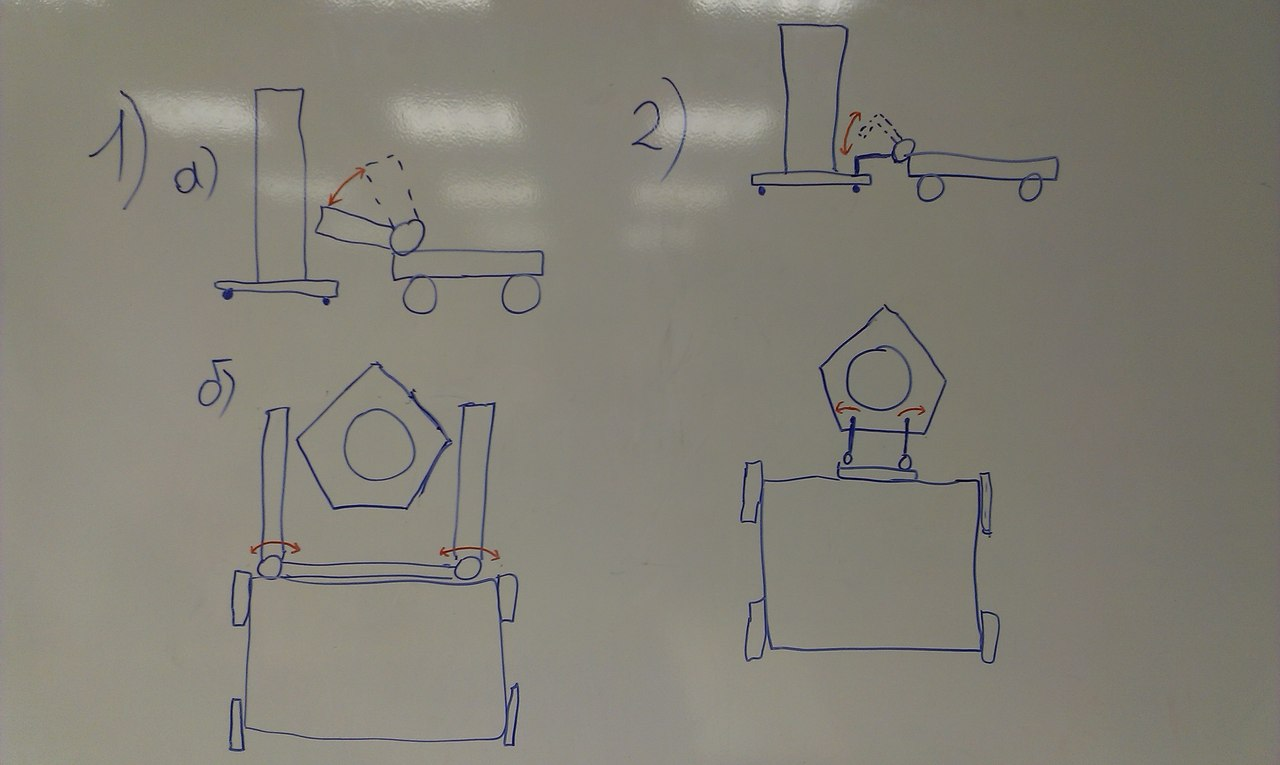
\includegraphics[scale=0.2]{days/08.11.14/images/01}}
					\caption{Ideas of capture of movable baskets: 1)Two beams 2)Vertical slats %-1 3)Клешни-2
						}
				\end{minipage}
			\end{figure}
			
		\end{enumerate}
		
		\item Since the mechanism of the trailer has not yet been selected, its assembly is not started.
		
		\item Because after it was decided to give up the idea capture mechanism baskets using servo turning the beam in the back parts of the robot is left unused hole, it was decided to adapt it under the socket of the power button.
		
		\begin{figure}[H]
			\begin{minipage}[h]{0.2\linewidth}
				\center  
			\end{minipage}
			\begin{minipage}[h]{0.6\linewidth}
				\center{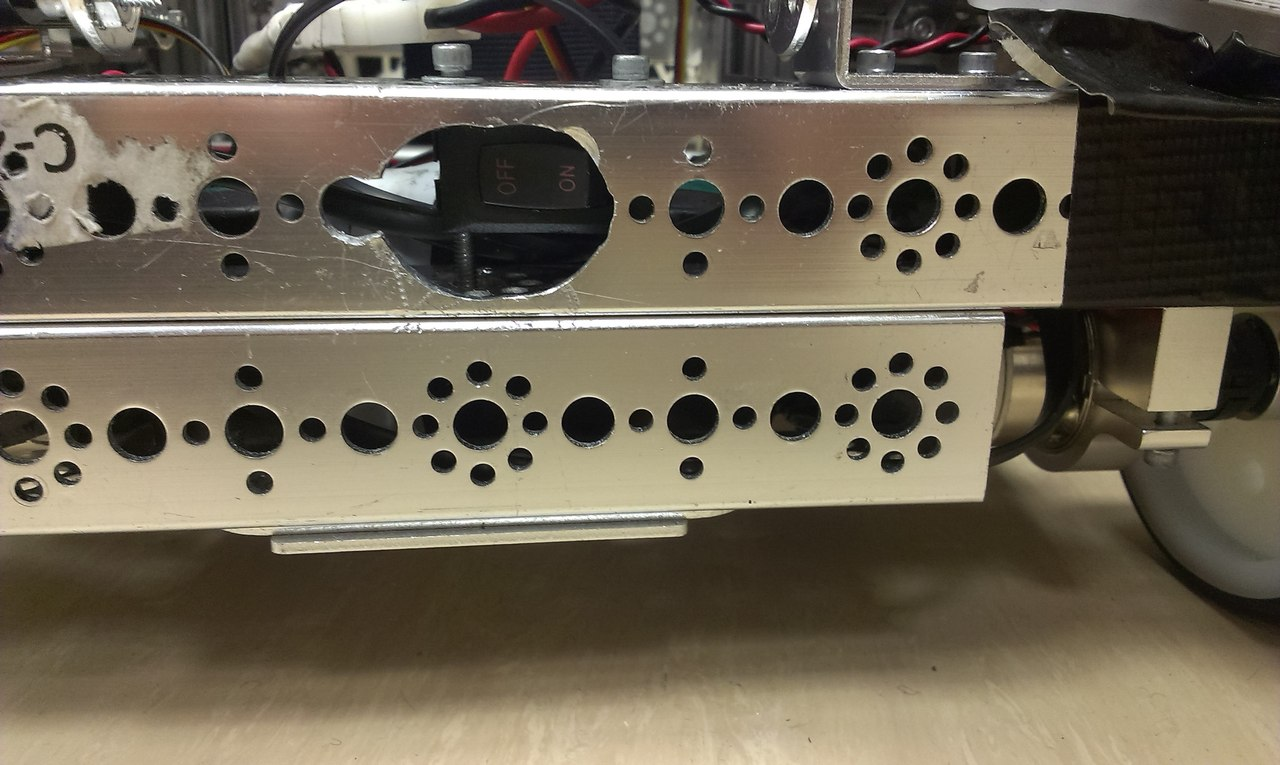
\includegraphics[scale=0.2]{days/08.11.14/images/02}}
				\caption{Button of power}
			\end{minipage}
		\end{figure}
		
	\end{enumerate}
	
	\item Results:  
	\begin{enumerate}
		\item Three ideas of design have been suggested.
		
		\item The mechanism of the trailer is not implemented.
		
	\end{enumerate}
	
	\item Tasks for the next congregations:
	\begin{enumerate}
		\item Choose the optimal variant of design capture mechanism.
		
		\item Gathering capture mechanism.
		
	\end{enumerate}     
\end{enumerate}
\fillpage

